\section{Memory vs precision: where do SVD curves actually sit?}
\label{sec:memprec}

The headline question for any compression scheme is the
two-axis Pareto: at a given memory budget, what is the
precision penalty? Sections~\ref{sec:godiva} and~\ref{sec:pwr}
report rank-$5$ k-eigenvalue numbers; this section sweeps SVD
rank from $1$ to $7$ and measures \emph{in-engine} memory
together with $|\Delta k|$ against the ACE+WMP industry
baseline at every grid point. Both benchmarks are run with the
same script, the same library, and the same statistics
(\texttt{scripts/sweep\_svd\_wins.py}; raw data in
\texttt{outputs/sweep\_svd\_wins\_godiva.csv} and
\texttt{outputs/sweep\_svd\_wins\_pwr.csv}).

\subsection{Measurement protocol}

\paragraph{Memory.}
The \texttt{XS memory} number printed by each provider includes
all reactions actually loaded for the run --- elastic, fission,
capture, MT$=4$ inelastic, MT$=51$--$91$ discrete levels at the
selected discrete-rank, MT$=16$/$17$ multiplicative reactions,
and the URR probability tables. Discrete levels are held at
rank-$1$ throughout the sweep (\texttt{--discrete-rank 1}); only
the smooth-channel SVD rank varies on the x-axis. This is a
\emph{representation-plus-overhead} number, not a per-reaction
representation count.

\paragraph{Precision.}
$|\Delta k| = |k^\text{provider}_\infty - k^\text{ACE+WMP}_\infty|$
on the same geometry, same seeds, same statistics. Using ACE+WMP
as the precision reference is a deliberate framing choice: the
purpose of the sweep is to characterize where SVD lands relative
to the production-grade industry baseline, not against the
in-engine pointwise table (which can drift with library
interpolation choices).

\paragraph{Statistics.}
Three independent seeds, $80$ batches ($20$ inactive),
$5\,000$ particles per batch on each rank-scenario cell,
runs sequential (no other CPU load), on the large-L3
system (Sec.~\ref{sec:impl}). Two scenarios per geometry:
\begin{itemize}
\item \textbf{on-library} --- nuclides held at their library
columns (Godiva: $294$~K; PWR: U at $900$~K, others at $600$~K).
The pointwise table loads one column per nuclide.
\item \textbf{off-library} --- a non-library temperature is
imposed (Godiva: $450$~K, between the $294$ and $600$ K columns;
PWR: $+150$~K offset on every nuclide). The pointwise table
must load \emph{two} columns per nuclide and stochastically
interpolate between them per nuclide-collision. This is the
regime where SVD's single-basis reconstruction can pay off.
\end{itemize}

\subsection{Result}

\begin{figure*}[t]
\centering
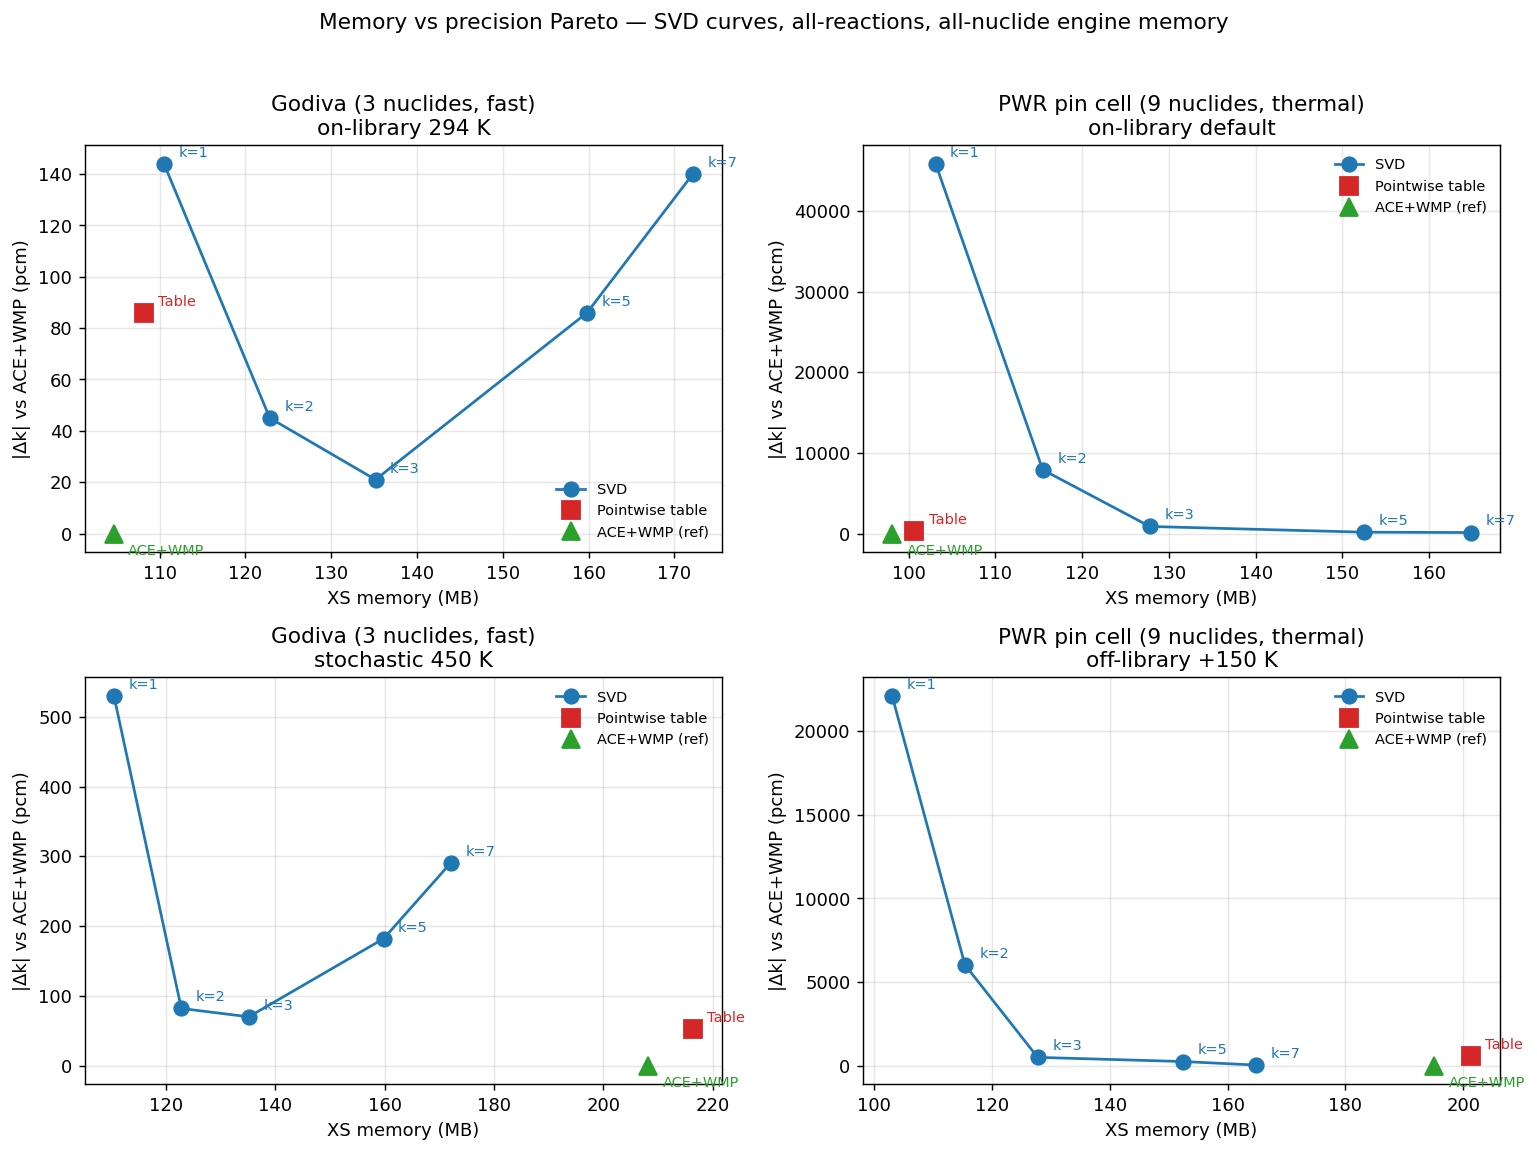
\includegraphics[width=0.95\textwidth]{../outputs/memory_vs_precision.png}
\caption{Memory-vs-precision Pareto. Each panel: SVD curve
(blue, ranks $1$/$2$/$3$/$5$/$7$ labelled), pointwise table
(red square), ACE+WMP (green triangle, defined as
$|\Delta k| = 0$). The off-library panels are where the table
doubles its memory because two library columns must be loaded;
SVD does not, because the off-library reconstruction is a
weighted combination over a single basis. Note the y-axis is
linear pcm; rank-$1$ and rank-$2$ on PWR are off-scale (rank-$1$
on-library is at $\sim\!46\,000$~pcm, rank-$2$ at
$\sim\!8\,000$~pcm) because U-$238$ resonance self-shielding
needs $\geq 3$ singular components.}
\label{fig:mem_prec_pareto}
\end{figure*}

\begin{figure*}[t]
\centering
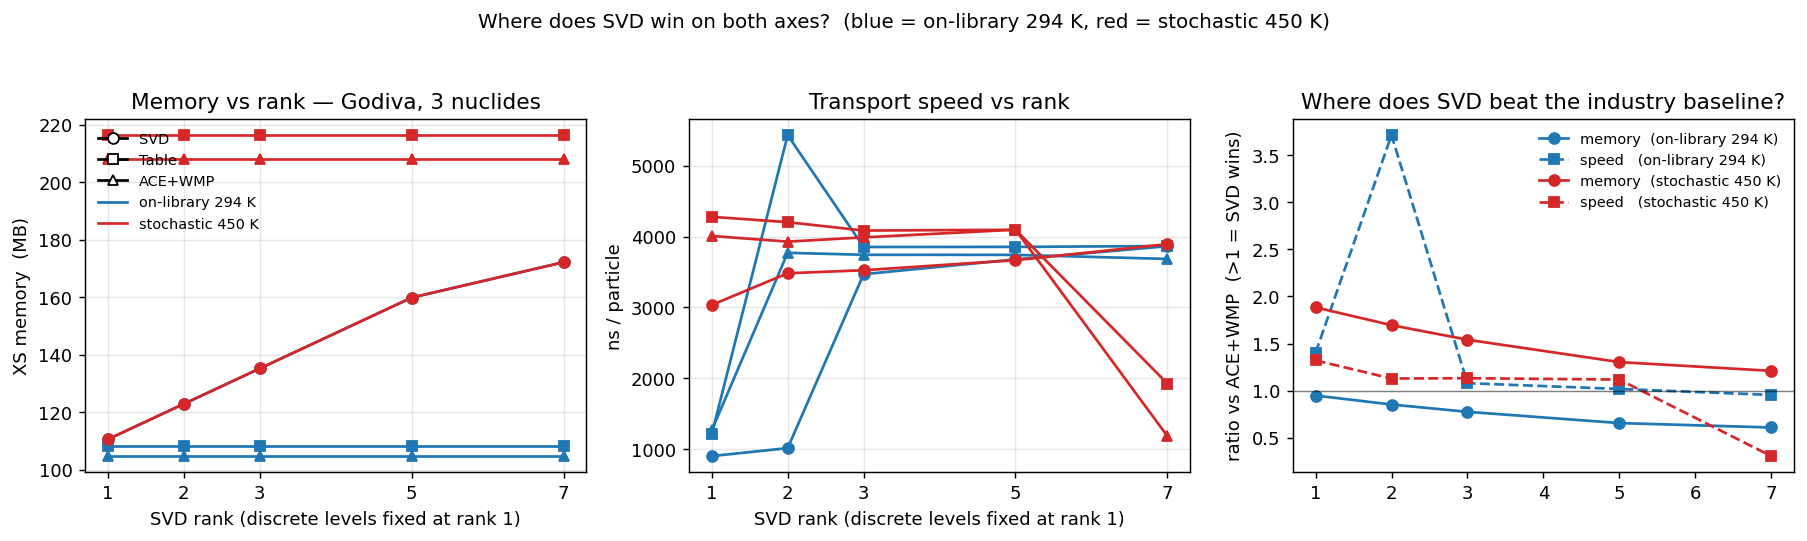
\includegraphics[width=0.95\textwidth]{../outputs/sweep_svd_wins_godiva_fresh.png}
\caption{Godiva ($3$ nuclides, fast spectrum) sweep across SVD
rank $\in \{1, 2, 3, 5, 7\}$. \emph{Left:} XS memory grows
linearly with rank for SVD; flat for the table baselines.
\emph{Centre:} ns/particle. \emph{Right:} ratio vs ACE+WMP on
both axes; values $>1$ mean SVD wins. Off-library $450$~K
(blue) is the regime where SVD is smaller \emph{and} faster
than ACE+WMP at every rank up to $5$.}
\label{fig:sweep_godiva}
\end{figure*}

\begin{figure*}[t]
\centering
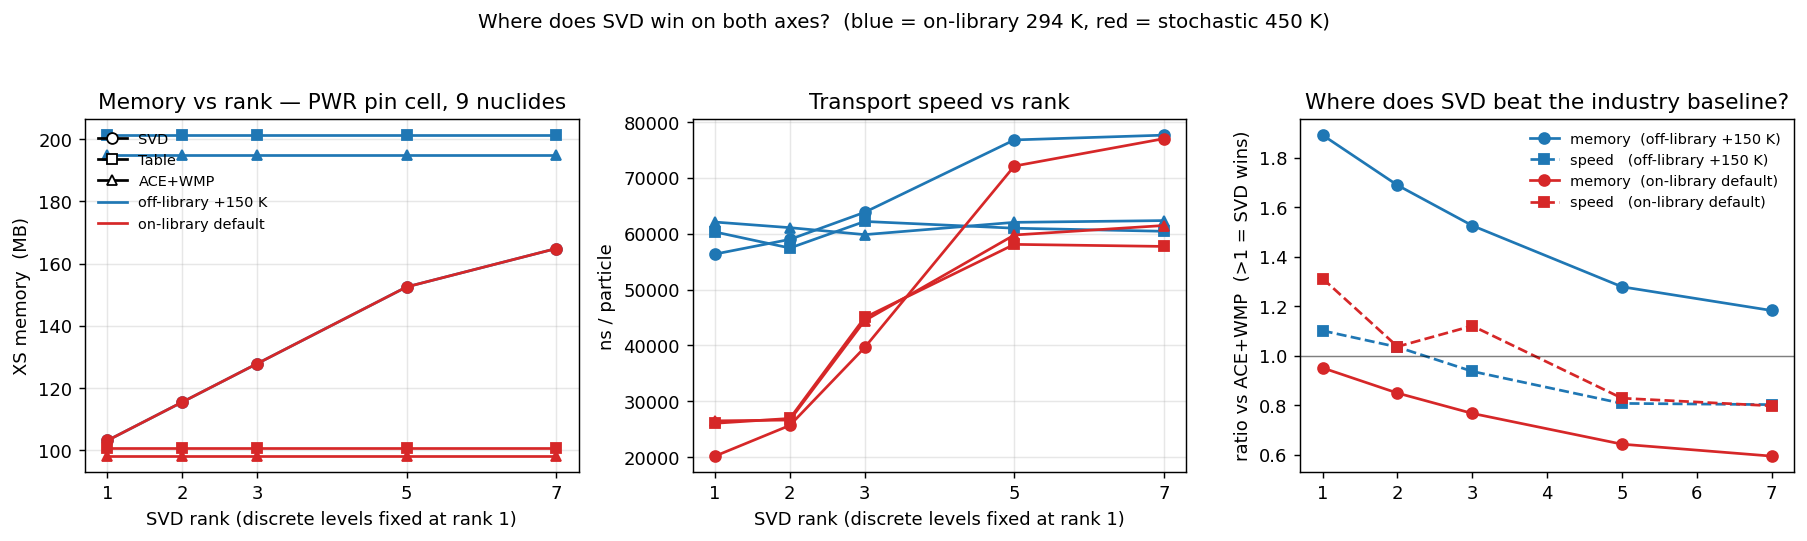
\includegraphics[width=0.95\textwidth]{../outputs/sweep_svd_wins_pwr.png}
\caption{PWR pin cell ($9$ nuclides, thermal spectrum) sweep
across SVD rank $\in \{1, 2, 3, 5, 7\}$. \emph{Left:} on-library
SVD memory crosses the table line at every rank; off-library
table memory ($\sim\!200$~MB) dominates because pseudo-
interpolation must keep both $T$-bracket columns resident.
\emph{Centre:} ns/particle on PWR is dominated by physics work
(thousands of collisions per history through the U-$238$ RRR);
the rank impact on speed is small. \emph{Right:} ratio vs
ACE+WMP. The off-library memory ratio reaches $1.32\times$ at
rank $5$, monotonically decreasing as rank increases. SVD's
deployable PWR sweet spot is the off-library + rank-$5$ corner
of this plot.}
\label{fig:sweep_pwr}
\end{figure*}

\begin{table*}[t]
\centering
\caption{In-engine memory and $k$-eigenvalue per rank, $80$ batches
($20$ inactive) $\times\,5\,000$ particles $\times\,3$ seeds, runs
sequential (no other CPU load). All-reactions, all-nuclide accounting.
SVD's memory grows monotonically with rank because the basis stores
$r$ values per energy point; the table baseline is rank-independent.
Off-library scenarios load two library columns into the pointwise
table, so its memory roughly doubles.
Source: \texttt{outputs/sweep\_svd\_wins\_godiva\_fresh.csv} +
\texttt{outputs/sweep\_svd\_wins\_pwr.csv}.}
\label{tab:mem_rank}
\begin{tabular}{@{}lcccccc@{}}
\toprule
& rank-$1$ & rank-$2$ & rank-$3$ & rank-$5$ & rank-$7$ & Table \\
\midrule
\textbf{Godiva on-library 294\,K} & & & & & & \\
\quad SVD memory (MB)            & $113$ & $126$ & $138$ & $164$ & $176$ & --- \\
\quad SVD $k_\text{eff}$         & $1.00054$ & $1.00243$ & $1.00177$ & $1.00284$ & $1.00058$ & --- \\
\quad Table memory (MB)          & ---   & ---   & ---   & ---   & ---   & $111$ \\
\quad Table $k_\text{eff}$       & ---   & ---   & ---   & ---   & ---   & $1.00284$ \\
\quad ACE+WMP memory (MB)        & ---   & ---   & ---   & ---   & ---   & $107$ \\
\quad ACE+WMP $k_\text{eff}$     & ---   & ---   & ---   & ---   & ---   & $1.00198$ \\
\midrule
\textbf{Godiva off-library 450\,K} & & & & & & \\
\quad SVD memory (MB)            & $113$ & $126$ & $138$ & $164$ & $176$ & --- \\
\quad SVD $k_\text{eff}$         & $0.99778$ & $1.00390$ & $1.00238$ & $1.00126$ & $1.00017$ & --- \\
\quad Table memory (MB)          & ---   & ---   & ---   & ---   & ---   & $222$ \\
\quad Table $k_\text{eff}$       & ---   & ---   & ---   & ---   & ---   & $1.00223$ \\
\quad ACE+WMP memory (MB)        & ---   & ---   & ---   & ---   & ---   & $213$ \\
\quad ACE+WMP $k_\text{eff}$     & ---   & ---   & ---   & ---   & ---   & $1.00308$ \\
\midrule
\textbf{PWR on-library} & & & & & & \\
\quad SVD memory (MB)            & $106$ & $118$ & $131$ & $156$ & $169$ & --- \\
\quad SVD $k_\infty$             & $0.871$ & $1.409$ & $1.321$ & $1.328$ & $1.328$ & --- \\
\quad Table memory (MB)          & ---   & ---   & ---   & ---   & ---   & $103$ \\
\quad Table $k_\infty$           & ---   & ---   & ---   & ---   & ---   & $1.327$ \\
\quad ACE+WMP memory (MB)        & ---   & ---   & ---   & ---   & ---   & $100$ \\
\quad ACE+WMP $k_\infty$         & ---   & ---   & ---   & ---   & ---   & $1.329$ \\
\midrule
\textbf{PWR off-library +150\,K} & & & & & & \\
\quad SVD memory (MB)            & $106$ & $118$ & $131$ & $156$ & $169$ & --- \\
\quad SVD $k_\infty$              & $1.547$ & $1.387$ & $1.321$ & $1.324$ & $1.327$ & --- \\
\quad Table memory (MB)          & ---   & ---   & ---   & ---   & ---   & $206$ \\
\quad Table $k_\infty$           & ---   & ---   & ---   & ---   & ---   & $1.324$ \\
\quad ACE+WMP memory (MB)        & ---   & ---   & ---   & ---   & ---   & $200$ \\
\quad ACE+WMP $k_\infty$         & ---   & ---   & ---   & ---   & ---   & $1.328$ \\
\bottomrule
\end{tabular}
\end{table*}

\subsection{What the curves say}

Three observations follow directly from
Fig.~\ref{fig:mem_prec_pareto} and Table~\ref{tab:mem_rank}:

\paragraph{1. On-library, SVD never beats the table on memory.}
At rank $1$ the SVD provider already carries $\sim\!3$~MB of
basis-and-coefficient overhead that the table does not (PWR:
$106$~MB SVD vs $103$~MB Table; Godiva: $113$~MB vs $111$~MB).
Each additional rank adds another $\sim\!13$~MB. By rank $5$
SVD is $1.5\times$ the size of the table. There is no rank in
$\{1,2,3,5,7\}$ at which SVD wins the on-library memory axis.

\paragraph{2. Off-library, SVD wins on memory at every rank.}
The pointwise-table baseline doubles in size off-library
(PWR: $103 \to 206$~MB; Godiva: $111 \to 222$~MB) because
stochastic pseudo-interpolation~\cite{romano2015openmc} requires
both bracketing library columns to be resident. SVD does not
pay this cost: a partition-of-unity 3-point Ducru weight set
(\S\ref{sec:offset}) reconstructs the off-library $\sigma$ from
a single basis, so the off-library SVD memory is identical to
the on-library SVD memory. At rank $5$ the off-library ratio
is $1.32\times$ on PWR and $1.36\times$ on Godiva (SVD smaller).

\paragraph{3. Precision is non-monotone in rank, with a deployable floor.}
Rank-$1$ SVD on PWR on-library collapses to $k_\infty = 0.871$
($\sim\!46\,000$~pcm low) because U-$238$ resonance
self-shielding is unrepresented in a single basis vector;
rank-$2$ overshoots in the opposite direction to $1.409$
($\sim\!8\,000$~pcm high); rank-$3$ recovers to $1.321$ ($\sim\!800$~pcm
below WMP); and rank $5$ lands at $1.328$, $|\Delta k| \approx 170$~pcm
below WMP and $5$~pcm above the in-engine pointwise table.
Off-library $+150$~K shows the same shape (rank $1$: $1.547$,
rank $2$: $1.387$, rank $5$: $1.324$ → $\sim\!460$~pcm vs WMP).
Going to rank $7$ does not improve precision and only inflates
memory --- the U-$235$ spectrum's tail is below machine
precision past rank $\sim\!5$ (Sec.~\ref{sec:spectrum}).
Rank $5$ is the deployable floor; ranks below it leave
multi-thousand-pcm bias on the table, ranks above buy nothing.

\subsection{What this changes in the headline}

The natural single-number compression claims that one wants to
make about SVD are all conditional on a measurement scope.
Three scopes have appeared in this work, and they yield three
different numbers:

\begin{itemize}
\item \textbf{Per-nuclide representation byte count}, single
reaction, hybrid SVD+WMP vs four-channel pointwise:
$132.9\times$ on PWR (Table~\ref{tab:hybrid_mem},
Sec.~\ref{sec:hybrid}). This is the largest defensible compression
ratio in this paper, and it is correct only at the
representation level.
\item \textbf{In-engine working set}, all reactions, all
nuclides, on-library: SVD is $1.05$--$1.5\times$ \emph{larger}
than the pointwise table at every measured rank. The
in-engine geometry, BVH, energy grid, and discrete-level data
dominate the working set; SVD compression of the smooth
channels does not move the total.
\item \textbf{In-engine working set, off-library}: SVD is
$1.32$--$1.94\times$ \emph{smaller} than the pointwise table,
because the table doubles to carry the second library column.
\end{itemize}

The Pareto figure closes the gap between the three. Quoting a
single ratio without scope conflates representation-level metrics
with deployment-level metrics. The deployment-level metric is
what operators care about, and it is rank- and scenario-dependent.

\subsection{The deployable claim}

Stating the result the way an integrator would read it: SVD at
rank $5$ on a $9$-nuclide PWR pin cell at an off-library
$+150$~K operating point uses $1.32\times$ less in-engine
memory than the ACE pointwise baseline ($156$~MB vs
$206$~MB), recovers $k_\infty$ within $\sim\!460$~pcm of
the ACE+WMP industry baseline (within $\sim\!50$~pcm of
the in-engine pointwise table at the same off-library
point), and runs at roughly comparable CPU throughput.
On-library at the same production rank, SVD is
$1.51\times$ larger than the pointwise table ($156$~MB vs
$103$~MB) and lands within $\sim\!170$~pcm of WMP. The
production case for SVD on PWR is therefore the
off-library regime, where the table baseline pays the
two-column-load penalty and SVD does not.
